\section{Erstellung des Sechobjects}

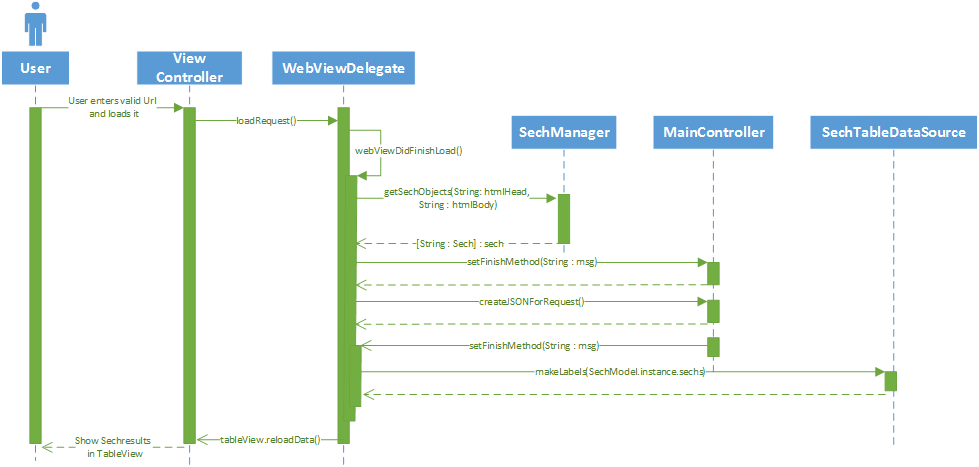
\includegraphics[scale=0.6]{sechobject.png}

%\textbf{Ablauf:}
Sobald der User eine gültige URL eingibt und lädt, wird die Laderoutine \Verb|loadRequest()|
angestoßen. Ist die Seite fertig geladen wird in der Delegatemethode \Verb|webViewDidFinishLoad()|
des WebViewDelegates das Auslesen bzw. Laden der \SEACH-Tags begonnen.

Dem \SEACH-Manager wird der HTML-Head und Body der eben geladenen Website übergeben und es
werden mit Hilfe des HTMLManagers \SEACH-Objekte erstellt. Diese \SEACH-Objekte werden in einem
Dictionary zurückgegeben.

Sobald ein Sechobject-Dictionary zurückgegeben wurde, werden die Ergebnisse gerankt und an den SechTableDataSource übergeben. Anschließend wird mit reloadData() die Tabelle der Sechtags im ViewController befüllt.
